\documentclass[preprint,12pt,a4paper]{elsarticle}

\usepackage{amssymb}
\usepackage{amsmath}
\usepackage{graphicx}
\usepackage{booktabs}
\usepackage{hyperref}
\usepackage{listings}
\usepackage{xcolor}
\usepackage{tikz}
\usepackage{multirow}
\usepackage{placeins}
\usepackage{float}
\usepackage{array}
\usepackage{tabularx}
\usepackage{microtype}
\usetikzlibrary{arrows.meta,positioning,shapes.geometric,fit,backgrounds,calc}

\lstset{
  language=Python,
  basicstyle=\ttfamily\footnotesize,
  keywordstyle=\color{blue},
  commentstyle=\color{gray},
  stringstyle=\color{red!70!black},
  frame=single,
  breaklines=true,
  captionpos=b,
}

\emergencystretch=2em
\setlength{\parindent}{0pt}
\setlength{\parskip}{0.5\baselineskip plus 2pt}

\journal{SoftwareX}

\begin{document}

\begin{frontmatter}

\title{\texttt{weatherisk}: A Python Package for Spatial Clustering
  of Climate Extremes via Max-Stable Processes}

\author[awi,uni]{Widad Kchikach\corref{cor1}}
\ead{widad.kchikach@awi.de}
\cortext[cor1]{Corresponding author}

\author[uni]{Thorsten Dickhaus}
\author[awi,uni]{Gerrit Lohmann}

\address[awi]{Alfred Wegener Institute Helmholtz Centre for Polar
  and Marine Research, Am Handelshafen 12, 27570 Bremerhaven, Germany}
\address[uni]{University of Bremen, Bibliothekstra\ss{}e 1,
  28359 Bremen, Germany}

\begin{abstract}
We present \texttt{weatherisk}, an open-source Python package for
identifying regions of homogeneous extremal dependence in gridded
climate-model output. The package implements a
complete analysis pipeline: an optional seasonal-trend decomposition
removes long-term trends from raw monthly fields; annual block maxima are
extracted, fitted with generalised extreme-value
distributions and transformed to the unit Fr\'{e}chet scale; local
spatial-dependence parameters are estimated; and grid cells are
partitioned into regions by Local Estimates Clustering or
Extremal Dependence Clustering. Its test suite compares it with
stored outputs of R code and runs without R. Revisiting a published
case study with the Alfred Wegener Institute (AWI)-ESM-1-1-LR
model, Extremal Dependence Clustering without detrending gives
the published 104~clusters and Local Estimates Clustering 23, against
24 published. With seasonal-trend detrending, which that study
reports, the counts are 142 and 14.
\end{abstract}

\begin{keyword}
spatial extremes \sep max-stable process \sep extremal dependence \sep spatial clustering \sep Python
\end{keyword}

\end{frontmatter}

\section*{Required Metadata}
\label{sec:metadata}

\section*{Current code version}

\begin{table}[H]
\small
\begin{tabularx}{\textwidth}{|l|>{\raggedright\arraybackslash}p{4.9cm}|>{\raggedright\arraybackslash}X|}
\hline
\textbf{Nr.} & \textbf{Code metadata description} & \textbf{Please fill in this column} \\
\hline
C1 & Current code version & v0.2.0 \\
\hline
C2 & Permanent GitHub link to code/repository used for this code version &
  \url{https://github.com/wkchikach99-byte/weatherisk/tree/v0.2.0} \\
\hline
C3 & Legal Code License & MIT License \\
\hline
C4 & Code versioning system used & git \\
\hline
C5 & Software code languages, tools, and services used &
  Python; SLURM (optional, for HPC runs) \\
\hline
C6 & Compilation requirements, operating environments
  \& dependencies &
  Python~$\geq$3.10 on Linux or macOS; NumPy; SciPy; pandas; matplotlib;
  Click; xarray; netCDF4; scikit-learn; Cartopy; h5py.
  Optional for development: pytest, pytest-cov, ruff, mypy, pyreadr,
  psutil, statsmodels. R is not required. The validation fixtures
  were generated once in R, with the R functions of Contzen
  et al., R's \texttt{stl()} and the scripts in
  \texttt{tests/}, and ship with the repository as frozen CSV and
  binary files. \\
\hline
C7 & If available Link to developer documentation/manual &
  \url{https://github.com/wkchikach99-byte/weatherisk\#readme} \\
\hline
C8 & Support email for questions & widad.kchikach@awi.de \\
\hline
\end{tabularx}
\caption{Code metadata (mandatory).}
\label{tab:metadata}
\end{table}

\section{Motivation and significance}
\label{sec:motivation}

Extreme weather events such as heavy precipitation or heat waves
rarely act on a single location; they typically unfold across broad
regions at once~\cite{davison2012}. While mean climate trends carry important information,
socioeconomic impacts are driven disproportionately by extreme events
rather than by shifts in average conditions~\cite{davison2012}. Infrastructure
failures, crop losses, and flood damage are governed by tail
probabilities (the chances of exceeding a rarely reached, very high
threshold)---not by means---of precipitation and temperature
distributions. Getting the tail behaviour and its spatial dependence
structure right is therefore central to any serious risk
quantification.

Extremes also behave differently from everyday climate
variability: they show non-Gaussian distributions, heavy
tails (where extreme values occur far more often than a bell-curve
distribution would predict), and extremal dependence---the
tendency for extreme events at different locations to co-occur%
---none of which standard
covariance-based techniques adequately represent~\cite{dehaan2006}. Extreme
value theory (EVT) provides the mathematical framework
for this regime. One standard approach in EVT is the
\emph{block maxima method}: the block maximum is the single largest
observed value within a fixed time window---here, one calendar year.
Under certain conditions, the distribution
of annual block maxima can be approximated well by a
\emph{generalised extreme-value} (GEV) distribution, a
three-parameter family~\cite{dehaan2006,padoan2010}. The family of GEV distributions contains the limiting
distribution of block-wise maxima for a broad range of data-generating
distributions. Capturing the
spatial dependence structure of these extremes across many grid
cells requires both a statistically sound framework and software
that can handle the associated computational burden---the dual
motivation for the present work.

\emph{Max-stable processes} are the standard framework for
modelling joint tail behaviour across space~\cite{dehaan2006,padoan2010}.
Following Contzen et al.~\cite{contzen2025}, fitting these models at each location
yields anisotropy parameters that capture the strength and
directional orientation of local spatial dependence.
Grid cells with similar parameter estimates can then be grouped
into \emph{clusters}---geographically connected regions in which
the extremal dependence structure is approximately uniform.

An R-based pipeline that implements this workflow was developed
by Contzen et al.~\cite{contzen2025}. It fits max-stable processes to given
climate datasets,
estimates local anisotropy parameters via pairwise composite
likelihood~\cite{padoan2010} (see Section~\ref{sec:architecture} for the
technical details), computes a pairwise dissimilarity score between
all grid cells based on the geometric overlap of their fitted
anisotropy ellipses, and groups cells by hierarchical clustering. Up
to now, however, the existing implementation is fragmented across independent
R scripts tied together by SLURM shell files. That implementation
served its intended purpose very well: it provided the empirical
illustration needed for the statistical methodology paper by Contzen
et al.~\cite{contzen2025}. As the method gains wider adoption and is applied to
larger or more varied datasets, however, a structured and installable
package becomes necessary, and that is precisely the gap
\texttt{weatherisk} fills.

\texttt{weatherisk} re-implements the full pipeline in a single
Python package that can be installed with \texttt{pip install} and is
tested against stored outputs of the R code
(Section~\ref{sec:validation}). It adds a preprocessing chain for
climate-model output, and checkpoint/restart support and parallel
execution for CMIP6 (Coupled Model Intercomparison
Project Phase~6)-style workloads on high-performance computing (HPC)
clusters.

Existing Python packages do support parts of the extreme-value workflow.
For example, \texttt{pyextremes}~\cite{pyextremes} and
\texttt{scikit-extremes}~\cite{scikitextremes}
focus on univariate extreme-value analysis, while the R package
\texttt{SpatialExtremes}~\cite{spatialextremes} provides max-stable simulation.
However, to our knowledge, no existing Python package offers the
integrated spatial-extremes workflow implemented here: max-stable
simulation, local composite-likelihood estimation, and ellipse-based
spatial clustering of extremes.

\section{Software description}
\label{sec:description}

\subsection{Software architecture}
\label{sec:architecture}

\texttt{weatherisk}~\cite{weatherisk} is a pip-installable Python package organised
into 22~modules and a command-line interface (CLI).  Figure~\ref{fig:workflow}
shows the overall workflow. The processing pipeline consists of six
stages:

\begin{enumerate}
\item \textbf{Preprocessing.}
  \begin{enumerate}
  \item[\textbf{(a)}] \textbf{STL decomposition (optional detrending).}
    Raw monthly precipitation series are decomposed with the STL
    (Seasonal-Trend decomposition using Loess) method of Cleveland
    et al.~\cite{cleveland1990}, in a NumPy translation of the
    Fortran routine that underlies R's \texttt{stl()} (module
    \texttt{stl}), with a 12-month period, a periodic seasonal
    component and robust fitting. This
    step removes the long-term trend from the series,
    leaving the seasonal cycle and interannual residuals available for
    extreme-value analysis. The step can be
    switched off (\texttt{detrend=False} in \texttt{CMIP6Config}).
  \item[\textbf{(b)}] \textbf{Annual block-maxima extraction.}
    From the monthly series, detrended or not, the annual maximum
    precipitation value is extracted for each grid cell, keeping
    only years for which observations are available in all 12 months.
    Taking the
    annual maximum thereby instantiates the block maxima
    approach of classical EVT~\cite{dehaan2006}.
  \item[\textbf{(c)}] \textbf{GEV fitting and Fr\'{e}chet
    transformation.}
    A GEV distribution is fitted independently at each grid cell
    by maximum likelihood. Each annual maximum is then mapped
    through the cell's fitted GEV cumulative distribution function and
    the inverse of the unit Fr\'{e}chet distribution function to the
    unit Fr\'{e}chet scale, the standard marginal scale of
    max-stable models.
    This puts all cells on an equal footing before spatial
    dependence is estimated: what remains captures where extremes
    co-occur, not how large they are at any individual site.
  \end{enumerate}
\item \textbf{Simulation} (for validation on synthetic data).
  Synthetic extremal-$t$ max-stable random fields with
  user-specified spatially varying anisotropy are generated on a
  regular grid by the spectral construction of
  Schlather~\cite{schlather2002}, with the positive parts of
  Gaussian spectral functions raised to the power~$\nu$, the degrees
  of freedom of the extremal-$t$ model, as in Opitz~\cite{opitz2013}.
\item \textbf{Local estimation.}
  For each grid cell, we estimate the three local anisotropy
  parameters of the extremal-$t$ dependence model of Contzen
  et al.~\cite{contzen2025,opitz2013}: the semi-minor axis length $a$
  of the anisotropy ellipse, the difference $b \ge 0$ between its
  semi-major and semi-minor axis lengths, and the rotation angle $\gamma$ of the
  semi-major axis. They are estimated by
  maximising a pairwise composite likelihood~\cite{padoan2010,contzen2025}. The
  optimisation runs over all neighbouring pairs within grid-point
  distance $\varepsilon$ (default $\varepsilon=5$ in \texttt{CMIP6Config}).
  The likelihood is maximised with the bounded quasi-Newton method
  L-BFGS-B from SciPy, started from 50 Latin-hypercube points
  (seed = 42).
\item \textbf{Spatial smoothing.}
  The raw estimates $(a_i, b_i, \gamma_i)$ (where
  subscript $i$ indexes the grid cell) are smoothed by a
  moving average over grid cells within a smoothing radius (default
  2.0 grid points in \texttt{CMIP6Config}).
\item \textbf{Clustering.}
  From the smoothed parameter estimates, we assemble a pairwise
  dissimilarity matrix and apply average-linkage hierarchical
  agglomerative clustering~\cite{contzen2025} to group grid cells into regions.
  Following Contzen et al.~\cite{contzen2025}, the number of
  clusters $k$ is the number of dendrogram merge heights that exceed
  a quantile of all pairwise dissimilarities (default:
  30\textsuperscript{th} percentile).
  Two dissimilarity measures are available:
  \begin{itemize}
  \item \textbf{LEC} (Local Estimates Clustering~\cite{contzen2025}; ellipse-overlap
    dissimilarity $D_2$): Jaccard-like overlap of the anisotropy
    ellipses (a ratio of intersection to union area, ranging
    from 0 for non-overlapping to 1 for identical ellipses; here
    used as a geometrically interpretable dissimilarity $1 - \text{overlap}$).
  \item \textbf{EDC} (Extremal Dependence Clustering~\cite{contzen2025}; madogram-based
    dissimilarity $D_1$, following Cooley et al.~\cite{cooley2006} and Saunders et al.~\cite{saunders2021}):
    the madogram is a rank-based, non-parametric summary of
    extremal dependence that maps onto pairwise extremal coefficients
    ranging from 1 (complete dependence) to 2
    (independence)~\cite{cooley2006}.
  \end{itemize}
\item \textbf{In-cluster re-estimation.}
  Within each cluster, one set of dependence parameters
  $(a,b,\gamma)$ is re-estimated from the data of all the cluster's
  grid cells by maximum pairwise composite likelihood (in the CMIP6
  pipeline, pairs up to $4.0\,\varepsilon$ apart and three starting
  points per cluster).
\end{enumerate}

\begin{figure}[ht]
\centering
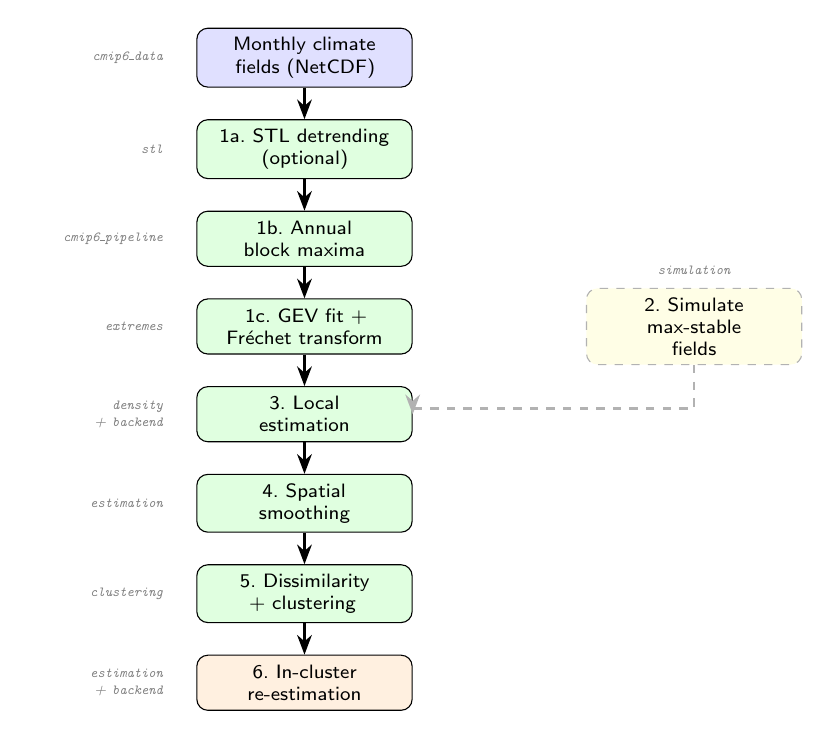
\begin{tikzpicture}[
  box/.style={draw, rounded corners=4pt, minimum width=2.6cm,
    minimum height=0.7cm, font=\sffamily\scriptsize,
    align=center, text width=2.5cm},
  data/.style={box, fill=blue!12},
  proc/.style={box, fill=green!12},
  outbox/.style={box, fill=orange!12},
  simbox/.style={box, fill=yellow!10, draw=gray!60, dashed},
  arr/.style={-{Stealth[length=2.5mm]}, thick},
  arrdashed/.style={-{Stealth[length=2.5mm]}, thick, dashed, gray!60},
  note/.style={font=\itshape\tiny, text=gray},
  node distance=0.4cm,
]

\node[data] (raw) {Monthly climate\\fields (NetCDF)};

\node[proc, below=of raw] (stl)
  {1a.\ STL detrending\\(optional)};
\node[proc, below=of stl] (bm)
  {1b.\ Annual\\block maxima};
\node[proc, below=of bm] (frech)
  {1c.\ GEV fit +\\Fr\'{e}chet transform};
\node[proc, below=of frech] (mle)
  {3.\ Local\\estimation};
\node[proc, below=of mle] (smooth)
  {4.\ Spatial\\smoothing};
\node[proc, below=of smooth] (clust)
  {5.\ Dissimilarity\\+ clustering};
\node[outbox, below=of clust] (out)
  {6.\ In-cluster\\re-estimation};

\draw[arr] (raw) -- (stl);
\draw[arr] (stl) -- (bm);
\draw[arr] (bm) -- (frech);
\draw[arr] (frech) -- (mle);
\draw[arr] (mle) -- (smooth);
\draw[arr] (smooth) -- (clust);
\draw[arr] (clust) -- (out);

\node[simbox, right=2.2cm of frech] (sim)
  {2.\ Simulate\\max-stable\\fields};
\node[note, above=0.05cm of sim, text width=2.5cm, align=center]
  {\texttt{simulation}};
\draw[arrdashed] (sim.south) -- ++(0,-0.55) -| (mle.east);

\node[note, left=0.3cm of raw, text width=1.6cm, align=right]
  {\texttt{cmip6\_data}};
\node[note, left=0.3cm of stl, text width=1.6cm, align=right]
  {\texttt{stl}};
\node[note, left=0.3cm of bm, text width=1.6cm, align=right]
  {\texttt{cmip6\_pipeline}};
\node[note, left=0.3cm of frech, text width=1.6cm, align=right]
  {\texttt{extremes}};
\node[note, left=0.3cm of mle, text width=1.6cm, align=right]
  {\texttt{density}\\+ \texttt{backend}};
\node[note, left=0.3cm of smooth, text width=1.6cm, align=right]
  {\texttt{estimation}};
\node[note, left=0.3cm of clust, text width=1.6cm, align=right]
  {\texttt{clustering}};
\node[note, left=0.3cm of out, text width=1.6cm, align=right]
  {\texttt{estimation}\\+ \texttt{backend}};

\end{tikzpicture}
\caption{Processing pipeline of \texttt{weatherisk}. Stage~1
  (a--c) is the preprocessing chain added for climate-model data;
  stage~1a can be switched off;
  stages~3--6 implement the core statistical methodology of Contzen
  et al.~\cite{contzen2025}. Module names are shown on the left. Stage~2
  (dashed box, right): \texttt{simulation.py} generates simulated
  max-stable fields on a regular 2-D grid with user-chosen dependence
  parameters (Schlather~\cite{schlather2002} spectral construction) and passes them to
  Stage~3 to check whether the pipeline gives back those known
  values.}
\label{fig:workflow}
\end{figure}

\subsection{Software functionalities}
\label{sec:functionalities}

\paragraph{Modules}
Figure~\ref{fig:workflow} names the module of each stage. The \texttt{covariance} module provides
the anisotropic, stationary or non-stationary correlation functions
of the extremal-$t$ dependence model and converts correlations into
extremal coefficients and back.

\paragraph{Scalability and execution (\texttt{cli})}
The command-line entry point
\texttt{weatherisk} has three sub-commands: \texttt{validate} for a
quick synthetic sanity check, \texttt{cmip6} for the case study of
Section~\ref{sec:ex-fig9} with STL detrending (the run without
detrending uses \texttt{scripts/reproduce\_fig9.py -{}-no-detrend}),
and \texttt{maps} for gridded observational data of the US National
Oceanic and Atmospheric Administration (NOAA) Climate Prediction
Center (CPC). The CMIP6 pipeline writes a checkpoint after each
stage, and after each cluster within the in-cluster re-estimation, so an
interrupted run resumes from the last completed unit of work.
SLURM scripts and setup are provided
under \texttt{hpc/}.

\paragraph{Computational cost}
The cost is dominated by the local estimation, the in-cluster
re-estimation, and the two dissimilarity matrices, whose $n(n-1)/2$
entries grow quadratically with the number of cells~$n$. The
simulation covariance and the ellipse overlaps are vectorised with
NumPy, and the per-cell and per-cluster optimisations run in
parallel worker processes.

\subsection{Validation}
\label{sec:validation}

\texttt{weatherisk} contains no R code and starts no R process. We
therefore establish its correctness by comparison with outputs of R
that were computed once and are stored in the repository
(\texttt{tests/reference\_data/}). They come from the R functions of
Contzen et al.~\cite{contzen2025}, evaluated on synthetic test cases
and on a simulated $10{\times}10$ field, and from an R workflow that
we wrote (\texttt{tests/generate\_cmip6\_mini\_reference.R}), which
combines these functions with R's \texttt{stl()} and runs the
climate pipeline, from detrending to clustering, on synthetic monthly
precipitation for a $5{\times}5$ grid and 20~years.

\textbf{Level~1: individual functions (116 tests).}
Each R function that \texttt{weatherisk} translates is compared with
its Python counterpart on identical inputs. Deterministic functions
must agree to absolute tolerances between $10^{-14}$ and $10^{-10}$;
on the simulated $10{\times}10$ field, the largest difference is
$1.4\times10^{-14}$. The STL module is compared with R's
\texttt{stl()} on 78~series in 14~configurations to a relative
tolerance of $10^{-12}$, with looser tolerances for one configuration
whose series consist mostly of exact zeros. The EDC dendrogram is the one result that is not
held to rounding error: many F-madogram distances on the
$10{\times}10$ field are tied, \texttt{hclust} and SciPy merge tied
pairs in a different order, and later merge heights differ by up to
$0.0032$. The threshold and the number of clusters equal R's
exactly, and 99.6\,\% of all pairs of cells are assigned
consistently (21 of 4{,}950 pairs differ).

\textbf{Level~2: the climate pipeline on synthetic data (16 tests).}
The synthetic data of the R workflow are run through the Python
pipeline, and each stage is compared with the stored R output
(Table~\ref{tab:pipeline-parity}). The local optimiser is judged by
likelihood: at each of the 25~cells, the pairwise negative
log-likelihood, summed over all neighbour pairs of the cell, may
exceed its value at R's optimum by at most~0.03. Equal parameters
are not a meaningful target, because each cell has 20~annual maxima
and, when $a$ is at its lower bound, the likelihood is nearly flat
in $b$ and $\gamma$. The Python value is lower than R's at 12~cells
(by up to $0.27$) and equal within $10^{-6}$ at the other 13. With
50 starts, the criterion held on these data and on five cells of the
simulated field for each of 21~seeds of the start design; with 20 or
40 starts, it failed for six and four of the seeds 0--9.

\textbf{Level~3: structure and regression (103 tests).}
These tests do not compare with R. They cover checkpointing and
resumption, equality of serial and parallel results, a static check
that the package source contains no R calls, the synthetic designs of
Contzen et al.~\cite{contzen2025}, and known regressions. With R
removed from the search path, all 235~tests pass in about 2\,min on
an Apple M4 laptop. Continuous integration runs the tests not marked
as slow under Python~3.10 and~3.11.

During validation we also found an indexing error in the LEC code of
the original R implementation. In the function
\texttt{calc\_distance\_ellipses} (\texttt{r\_code/functions.R},
line 515 in the repository version used here; see
\url{https://github.com/wkchikach99-byte/weatherisk/blob/4cf18b2/r_code/functions.R\#L515}),
the branch for an empty ellipse inside the loop over the grid-cell
indices \texttt{i} and \texttt{j} assigns \texttt{dist\_matrix[j] = 1}
instead of \texttt{dist\_matrix[i,j] <- 1}. R reads the single index as a linear index, so the value is written
to the wrong entry of the dissimilarity matrix without an error.
\texttt{weatherisk} implements the intended assignment; the
validation test replays the R behaviour.

\begin{table}[!htbp]
\centering
\small
\setlength{\tabcolsep}{4pt}
\begin{tabularx}{\textwidth}{>{\raggedright\arraybackslash}p{3.6cm}>{\raggedright\arraybackslash}X>{\raggedright\arraybackslash}p{3.0cm}}
\toprule
\textbf{Stage} & \textbf{Criterion} & \textbf{Largest deviation} \\
\midrule
STL detrending & absolute $\leq 10^{-13}\max|x|$ & \mbox{$2.3{\times}10^{-14}\max|x|$} \\
Annual maxima & relative $\leq 10^{-12}$ & $2.0\times10^{-14}$ \\
GEV fit, Fr\'{e}chet & absolute $\leq 10^{-3}$; relative $\leq 2\times10^{-3}$ & $4.2\times10^{-4}$; $9.6\times10^{-4}$ \\
Local estimation & $\mathrm{NLL}_{\text{Python}} \leq \mathrm{NLL}_{\text{R}} + 0.03$ & $+7.3\times10^{-7}$ \\
Ellipse overlap & absolute $10^{-14}$ plus relative $5\times10^{-15}$ & $1.9\times10^{-15}$ \\
LEC clustering & threshold within $10^{-14}$, $k$ equal & $k$ equal \\
EDC madogram & absolute $\leq 10^{-10}$ & $5\times10^{-16}$ \\
EDC clustering & threshold within $10^{-12}$, $k$ equal & $k$ equal \\
\bottomrule
\end{tabularx}
\caption{Level~2 comparison with the R workflow. $x$ is the monthly
  series; NLL is the pairwise negative log-likelihood of a cell; GEV
  parameters and Fr\'{e}chet margins are separated by a semicolon.}
\label{tab:pipeline-parity}
\end{table}

\section{Illustrative examples}
\label{sec:examples}

\subsection{Example~1: Synthetic validation}
\label{sec:ex-synthetic}

We simulate 250 replicates of extremal-$t$ max-stable data on a
51$\times$51 grid where the axis difference $b = (x+5)/2$ increases
linearly from 0 on the left to 5 on the right, while $a = 2$ and
$\gamma = 0$ are constant, creating vertical ``stripe'' regions. The call
\texttt{run\_nonstationary\_pipeline("paper\_stripes", seed=42,
n\_workers=32)} took 8.4~hours of wall
time. The preset
sets $\varepsilon$ and the smoothing radius to 4 grid points, and the
in-cluster re-estimation uses pairs up to 4 grid points apart.

Figure~\ref{fig:stripes} shows the result. The in-cluster estimates
of~$b$ of the seven EDC clusters range from 0.31 to 3.73 and follow
the left-to-right trend, but no column of the grid lies within a single EDC
cluster. Four of the five LEC clusters are vertical bands, with
in-cluster estimates $b = 0.37$, 1.68, 3.42 and 4.60 from left to
right; the fifth is a cluster of 28~cells in the upper-right corner
($b = 5.07$). Of the 51~grid columns, 24 lie entirely within one LEC
cluster. If each cell is assigned the estimate of its cluster, the
mean absolute error with respect to the true~$b$ over the 2601~cells
is 0.37 for LEC and 0.86 for EDC. Contzen et al.\ report the same
contrast for this design (Fig.~3 in~\cite{contzen2025}). They obtain six clusters with both
methods. The counts need not agree, because the Python package draws
the 250 replicates with its own random number generator.

\begin{figure}[!htbp]
\centering
\includegraphics[width=0.95\textwidth]{figures/fig3_stripes.png}
\caption{Synthetic validation on the ``stripes'' preset
  (seed~42, $k_{\text{edc}} = 7$, $k_{\text{lec}} = 5$).
  (a)~EDC clusters coloured by their estimated axis difference~$b$;
  (b)~LEC clusters coloured by their estimated~$b$;
  (c)~true field $b = (x+5)/2$, rising from 0 to~5.
  The LEC boundaries are mostly vertical, as in the true field;
  several EDC boundaries run horizontally.}
\label{fig:stripes}
\end{figure}

\FloatBarrier

\subsection{Example~2: Revisiting the published case study --- AWI-ESM-1-1-LR
  global precipitation}
\label{sec:ex-fig9}

We revisit the Figure~9 analysis of Contzen et al.~\cite{contzen2025} with
monthly precipitation from the AWI-ESM-1-1-LR
historical simulation (T63 grid, $192 \times 96$ cells, r1i1p1f1,
years 1850--2005) and the parameter settings of
Table~\ref{tab:fig9-params}. The pipeline was run twice on one
64-core node of the Alfred Wegener Institute (AWI)
\emph{albedo} HPC cluster, as two jobs of the SLURM script
\texttt{hpc/run\_fig9\_pyonly.slurm}, each running one command of
Listing~\ref{lst:fig9}.

\begin{table}[ht]
\centering
\begin{tabular}{ll}
\toprule
\textbf{Parameter} & \textbf{Value} \\
\midrule
Degrees of freedom $\nu$ & 5 \\
Covariance exponent $\alpha$ & 1 \\
Neighbour radius $\varepsilon$ & 5 (grid-point units) \\
Clustering quantile threshold & 30\textsuperscript{th} percentile \\
Period & 1850--2005 (156~years) \\
\bottomrule
\end{tabular}
\caption{Parameter settings used for the case study of Example~2,
  following Section~5 of Contzen et al.~\cite{contzen2025}.}
\label{tab:fig9-params}
\end{table}

\begin{lstlisting}[caption={Running the case study of Example~2 on HPC.},
  label=lst:fig9, numbers=none]
$ python scripts/reproduce_fig9.py \
    --data-dir /path/to/AWI-ESM-1-1-LR/pr/ \
    --workers 64  --output-dir output/fig9_detrend
$ python scripts/reproduce_fig9.py \
    --data-dir /path/to/AWI-ESM-1-1-LR/pr/ \
    --workers 64  --output-dir output/fig9_nodetrend \
    --no-detrend
\end{lstlisting}

With and without STL detrending, local estimation took 11.9\,h and
11.8\,h, both dissimilarity matrices together about 5\,min, and the
in-cluster re-estimation 24\,h and 14\,h; stages 3--6, resumed from
the checkpoint after stage~1, took 36.0\,h and 26.0\,h of wall time.
The re-estimation assigns one worker to each cluster, so the last
clusters to finish ran on single workers while most cores were idle,
and the CPU utilisation averaged 35\% and 47\% of the 64 cores. The
largest single process peaked at 36\,GiB and 38\,GiB of resident
memory.

\begin{table}[ht]
\centering
\begin{tabular}{lcc}
\toprule
\textbf{Run} & \textbf{EDC ($k_{\text{edc}}$)} &
  \textbf{LEC ($k_{\text{lec}}$)} \\
\midrule
Contzen et al.~\cite{contzen2025} & 104 & 24 \\
\texttt{weatherisk}, no detrending & 104 & 23 \\
\texttt{weatherisk}, STL detrending & 142 & 14 \\
\bottomrule
\end{tabular}
\caption{Cluster counts for the case study of Example~2 (30\% quantile
  threshold in all cases).}
\label{tab:fig9-counts}
\end{table}

Table~\ref{tab:fig9-counts} and Figure~\ref{fig:fig9} show the
results. Contzen et al.~\cite{contzen2025} state that the data were
detrended with STL, but they do not report the STL settings. We therefore cannot tell which
preprocessing produced the published counts, and we report both
runs.

The EDC chain involves no numerical optimisation, since the
madogram depends only on the ranks of the annual maxima. For six
STL variants (seasonal component also removed, non-robust fitting,
\texttt{s.window} of 7 or 13, period extended to 2014, and the
setting above), $k_{\text{edc}}$ lay between 137 and 147 with the
merge orders of SciPy and of R's \texttt{hclust}; without
detrending, it was 104 and 106. Such differences come from the order
in which equal dissimilarities are merged. For the STL input, the R
functions of Contzen et al.\ give 140, and permuting tied entries
gives 139 to 142.

The LEC count also depends on the local estimates and hence on the
optimiser. Where the likelihood is flat, optima of equal likelihood
can have different parameters (Section~\ref{sec:validation}), so we
do not interpret the difference between 23 and 24. Both runs used
commit \texttt{7561a6e}; recomputing their EDC labels with the only
later change to the computation, R's rank rule for tied annual maxima
in the madogram,
gives identical labels.

\FloatBarrier
\begin{figure}[!htbp]
\centering
\includegraphics[width=\textwidth]{figures/fig9_pyonly_comparison.png}
\caption{The case study of Contzen
  et al.~\cite{contzen2025} (their Figure~9) recomputed with \texttt{weatherisk}: EDC clusters
  (left) and LEC clusters (right) of annual maxima of monthly
  AWI-ESM-1-1-LR historical precipitation (T63 grid, 1850--2005;
  $\nu = 5$, $\alpha = 1$, $\varepsilon = 5$, 30\% quantile
  threshold), computed without detrending (top row) and with STL
  detrending (bottom row). Colours only distinguish clusters within a
  panel and are reused when a panel has more clusters than colours.}
\label{fig:fig9}
\end{figure}

\FloatBarrier

\section{Impact}
\label{sec:impact}

The core output of \texttt{weatherisk} is a partition of the
grid into spatially coherent regions, far fewer than the grid cells, each characterised by a common extremal
dependence structure. Working with these regions rather than
thousands of individual grid cells makes the analysis tractable and
raises concrete applied questions: which areas share a common
extreme-precipitation hazard, how do hazard boundaries shift across
climate states, and where should spatial risk aggregation be drawn
in insurance or infrastructure planning?

The test suite of Section~\ref{sec:validation} lets a user check an
installation against stored outputs of R without installing R.

The pairwise dissimilarity matrix has $n^2$ entries for $n$
grid cells, and this quadratic cost remains the main limit on grid
size.
One methodological limitation of the present framework is
its reliance on block maxima: only the largest value per year
and grid cell is used, so further extremes within the same year do
not enter the analysis. Future work could explore peaks-over-threshold
(POT) extensions in a spatial setting~\cite{davison2012}, which use
more of the data within the same theoretical framework.

\paragraph{New research directions}
The Python API and the command-line interface can be applied to
other variables (for example wind speed or sea-level pressure) and
other datasets (for example ERA5 or CMIP6 projections). These
applications are not tested in this paper.

\paragraph{Education}
The step-by-step pipeline, the test suite and the code examples in
the repository README can be used to teach spatial extreme-value
analysis. The Jupyter notebook
\texttt{notebooks/\allowbreak weatherisk\_quickstart.ipynb} runs a
lightweight synthetic check without local estimation.

\section{Conclusions}
\label{sec:conclusions}

We have presented \texttt{weatherisk}, a Python package that
implements the complete pipeline for spatial clustering of climate
extremes via max-stable processes. Its tests compare it with
stored outputs of R function by function and, on synthetic data,
stage by stage, without calling R. Stages 3--6 of the
case study on the AWI-ESM-1-1-LR T63 grid took 26 to 36~hours
on 64~cores. Without detrending it reproduces the published EDC count
of 104 and gives 23 LEC clusters against 24; the dependence of the
counts on detrending (Section~\ref{sec:ex-fig9}) shows that the
preprocessing has to be reported with the clustering.

The clusters condense a large climate field into a small set of
regions in which extremes co-occur. Such regions are the spatial units
needed for risk aggregation in reinsurance, infrastructure planning,
and climate services.

\paragraph{Outlook: Digital Earth System Twins}
High-resolution digital replicas of the Earth system, such as those
being developed in the European Destination Earth
initiative~\cite{bauer2021}, will require automated analysis tools
that operate at the same scale and cadence.
Spatial clustering of extremes could be one step in such a pipeline,
converting per-cell dependence estimates into a small set of
homogeneous regions that can be passed to impact models.
Future extensions would require incremental cluster updating, linkage
to socioeconomic exposure databases, and objective criteria for
detecting structural regime shifts.

\texttt{weatherisk} is available under the MIT licence.

\section*{CRediT authorship contribution statement}
\textbf{Widad Kchikach:} Methodology, Software, Validation,
Investigation, Visualization, Writing -- original draft.
\textbf{Thorsten Dickhaus:} Conceptualization, Supervision,
Writing -- review \& editing.
\textbf{Gerrit Lohmann:} Conceptualization, Supervision,
Writing -- review \& editing.

\section*{Declaration of Competing Interests}

The authors declare that they have no known competing financial
interests or personal relationships that could have appeared to
influence the work reported in this paper.

\section*{Data availability}
The AWI-ESM-1-1-LR historical simulation used in
Section~\ref{sec:ex-fig9} is publicly available from the Earth
System Grid Federation~\cite{danek2020}. The synthetic data of
Section~\ref{sec:ex-synthetic} are generated by the package from the
seed given there.

\section*{Declaration of generative AI and AI-assisted technologies in the manuscript preparation process}
During the preparation of this work the authors used Claude
(Anthropic) to assist with writing and testing code and
with editing the manuscript text. After using this tool, the
authors reviewed and edited the content as needed and take full
responsibility for the content of the published article.

\section*{Acknowledgements}
The authors thank the Alfred Wegener Institute Helmholtz Centre for
Polar and Marine Research (AWI) for access to the \emph{albedo}
computing cluster, on which the case study of Example~2 was run. We thank J.~Contzen for the original R implementation of
the methods, on which \texttt{weatherisk} is based.

\paragraph*{Funding}
This work was supported by the Helmholtz Association [grant number
HIDSS-0005, MarDATA Helmholtz School for Marine Data Science] and the
European Research Council [ERC Synergy Grant i2B, grant number
101118519]. The funders had no role in study design; in the
collection, analysis and interpretation of data; in the writing of
the report; or in the decision to submit the article for
publication.

\begin{thebibliography}{00}

\bibitem{davison2012}
A.C.~Davison, S.A.~Padoan, M.~Ribatet,
Statistical modeling of spatial extremes,
Stat.\ Sci.\ 27\,(2) (2012) 161--186.
\url{https://doi.org/10.1214/11-STS376}

\bibitem{dehaan2006}
L.~de~Haan, A.~Ferreira,
Extreme Value Theory: An Introduction,
Springer, New York, 2006.
\url{https://doi.org/10.1007/0-387-34471-3}

\bibitem{padoan2010}
S.A.~Padoan, M.~Ribatet, S.A.~Sisson,
Likelihood-based inference for max-stable processes,
J.\ Am.\ Stat.\ Assoc.\ 105\,(489) (2010) 263--277.
\url{https://doi.org/10.1198/jasa.2009.tm08577}

\bibitem{contzen2025}
J.~Contzen, T.~Dickhaus, G.~Lohmann,
Regionalization approaches for the spatial analysis of extremal
dependence,
Extremes 28\,(4) (2025) 713--737.
\url{https://doi.org/10.1007/s10687-025-00519-2}

\bibitem{pyextremes}
[software] G.~Bocharov,
pyextremes: Extreme value analysis in Python, version 2.6.1,
\url{https://github.com/georgebv/pyextremes} [accessed 14
November 2026].

\bibitem{scikitextremes}
[software] K.~Correoso,
scikit-extremes: univariate extreme value analysis in Python,
\url{https://github.com/kikocorreoso/scikit-extremes}
[accessed 14 November 2026].

\bibitem{spatialextremes}
[software] M.~Ribatet,
SpatialExtremes: Modelling Spatial Extremes,
R package version 2.1-0, 2022, archived on CRAN,
\url{https://doi.org/10.32614/CRAN.package.SpatialExtremes}.

\bibitem{weatherisk}
[software] W.~Kchikach, T.~Dickhaus, G.~Lohmann,
weatherisk: A Python Package for Spatial Clustering of Climate
Extremes via Max-Stable Processes, version 0.2.0, Zenodo (2026),
\url{https://doi.org/10.5281/zenodo.XXXXXXX}.

\bibitem{cleveland1990}
R.B.~Cleveland, W.S.~Cleveland, J.E.~McRae, I.~Terpenning,
STL: A seasonal-trend decomposition procedure based on loess,
J.\ Off.\ Stat.\ 6\,(1) (1990) 3--73.

\bibitem{schlather2002}
M.~Schlather,
Models for stationary max-stable random fields,
Extremes 5\,(1) (2002) 33--44.
\url{https://doi.org/10.1023/A:1020977924878}

\bibitem{opitz2013}
T.~Opitz,
Extremal $t$ processes: Elliptical domain of attraction and a
spectral representation,
J.\ Multivar.\ Anal.\ 122 (2013) 409--413.
\url{https://doi.org/10.1016/j.jmva.2013.08.008}

\bibitem{cooley2006}
D.~Cooley, P.~Naveau, P.~Poncet,
Variograms for spatial max-stable random fields,
in: P.~Bertail, P.~Soulier, P.~Doukhan (Eds.),
Dependence in Probability and Statistics,
Springer, 2006, pp.~373--390.
\url{https://doi.org/10.1007/0-387-36062-X_17}

\bibitem{saunders2021}
K.~Saunders, A.G.~Stephenson, D.J.~Karoly,
A regionalisation approach for rainfall based on extremal dependence,
Extremes 24\,(2) (2021) 215--240.
\url{https://doi.org/10.1007/s10687-020-00395-y}

\bibitem{bauer2021}
P.~Bauer, B.~Stevens, W.~Hazeleger,
A digital twin of Earth for the green transition,
Nat.\ Clim.\ Change 11\,(2) (2021) 80--83.
\url{https://doi.org/10.1038/s41558-021-00986-y}

\bibitem{danek2020}
[dataset] C.~Danek, X.~Shi, C.~Stepanek, H.~Yang, D.~Barbi,
J.~Hegewald, et~al.,
AWI AWI-ESM1.1LR model output prepared for CMIP6 CMIP historical,
version 20200212, Earth System Grid Federation (2020),
\url{https://doi.org/10.22033/ESGF/CMIP6.9328}.

\end{thebibliography}

\end{document}
